% This is samplepaper.tex, a sample chapter demonstrating the
% LLNCS macro package for Springer Computer Science proceedings;
% Version 2.20 of 2017/10/04
%
\documentclass[runningheads]{llncs}
%
\usepackage{graphicx}
\usepackage{cite}
% Used for displaying a sample figure. If possible, figure files should
% be included in EPS format.
%
% If you use the hyperref package, please uncomment the following line
% to display URLs in blue roman font according to Springer's eBook style:
% \renewcommand\UrlFont{\color{blue}\rmfamily}

\begin{document}
%
\title{Rule Driven Query Expansion}
%
%\titlerunning{Abbreviated paper title}
% If the paper title is too long for the running head, you can set
% an abbreviated paper title here
%
\author{Xinze Lyu \and
Wei Hu}
%
\authorrunning{F. Author et al.}
% First names are abbreviated in the running head.
% If there are more than two authors, 'et al.' is used.
%
\institute{State Key Laboratory for Novel Software Technology, Nanjing University, China \and
Department of Computer Science and Technology, Nanjing University, China
\email{xzlv.nju@gmail.com, whu@nju.edu.cn}\\
}
%
\maketitle              % typeset the header of the contribution
%
\begin{abstract}
  Empty answers problem exists when we use SPARQL to access RDF knowledge graph data. Put situations that querying facts inexistent to the real world aside, one reason is that users lack enough knowledge for a particular RDF knowledge graph, that leads to SPARQL queries with wrong formats or inaccurate expressions.  However, due to the schema-free nature of RDF data and incompleteness of particular RDF knowledge graphs, even a SPARQL query with correct format can reflect users' intentions accurately, it may fail to get any results. Researches going on in translating the natural language to SPARQL help a lot to address the first problem, but these are inconducive for the second problem which was caused by the faults in structure and content of RDF knowledge graphs.
  We design a rule-driven framework to alleviate the obstacles caused by the structure and content of RDF knowledge graphs. Specifically, given a SPARQL query, we use knowledge graph oriented rule-learning procedure to take reasoning rules, with the help of these rules, our system return possible results. More importantly, our system shows detailed information with similarity score and rules to explain why our system chooses particular possible answers.
\keywords{SPARQL  \and Empty Answer \and Rule Learning.}
\end{abstract}
%
%
%
\section{Problem Statement}
\subsection{Empty Answer Problem for SPARQL query}
Users use SPARQL queries reflecting their intentions to access the  data from RDF knowledge graph, reasons for Empty Answer Problem are various, three of which are main ones, 1)the facts that users want to query  do not exist in the real world; 2)the formats of SPARQL is wrong, including  the namespace, operators and so on; 3)SPARQL queries are accurate and well-formatted, but they do not have exact matches in particular RDF knowledge graphs.

We focus on the third one.  There are two factors that contribute to the third problems. One is the SPARQL queries have a high level of constraints, we get an instance from the released resource of ~\cite{wangEmbed}, there are three constraints for SPARQL query in table ~\ref{S_Example}. This query gets no answers, in fact, the constraints (1) and (2) are redundant, we can infer that ``?company" is dbr:Apple\_Inc with constraints (3).

\begin{table}
\caption{SPARQL query with high constraints.}\label{S_Example}
\centering
\begin{tabular}{|c|c|}
\hline
\multicolumn{2}{|l|}{SELECT ?company WHERE }\\
\hline
(1) &  ?company rdfs:type dbo:Company.\\
(2) &  ?company dbo:industry dbr:Electronics.\\
(3) & dbr:IPhone dbp:developer ?company.\\
\hline
% \multicolumn{2}{|c|}{}}\\
% \hline
\end{tabular}
\end{table}
% \subsubsection{Sample Heading (Third Level)}
% \paragraph{Sample Heading (Fourth Level)}
\subsection{Semantic Parsing}
\subsection{Paraphrasing}
\subsection{Similarity Based Method}
\subsection{Ontology Rule Based Method}
\subsection{Embedding Based Method}

\begin{table}
\caption{Table captions should be placed above the
tables.}\label{tab1}
\begin{tabular}{|l|l|l|}
\hline
Heading level &  Example & Font size and style\\
\hline
Title (centered) &  {\Large\bfseries Lecture Notes} & 14 point, bold\\
1st-level heading &  {\large\bfseries 1 Introduction} & 12 point, bold\\
2nd-level heading & {\bfseries 2.1 Printing Area} & 10 point, bold\\
3rd-level heading & {\bfseries Run-in Heading in Bold.} Text follows & 10 point, bold\\
4th-level heading & {\itshape Lowest Level Heading.} Text follows & 10 point, italic\\
\hline
\end{tabular}
\end{table}


\noindent Displayed equations are centered and set on a separate
line.
\begin{equation}
x + y = z
\end{equation}
Please try to avoid rasterized images for line-art diagrams and
schemas. Whenever possible, use vector graphics instead (see
Fig.~\ref{fig1}).

\begin{figure}
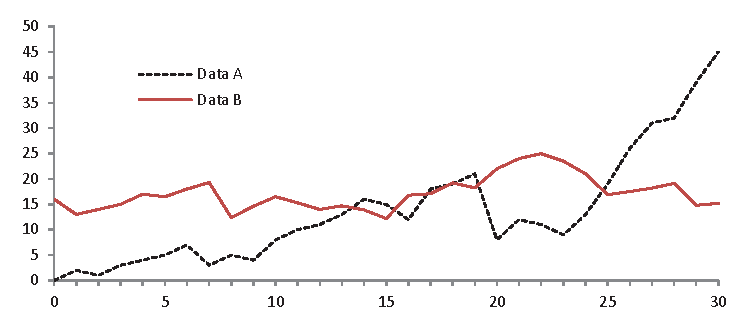
\includegraphics[width=\textwidth]{fig1.eps}
\caption{A figure caption is always placed below the illustration.
Please note that short captions are centered, while long ones are
justified by the macro package automatically.} \label{fig1}
\end{figure}

\begin{theorem}
This is a sample theorem. The run-in heading is set in bold, while
the following text appears in italics. Definitions, lemmas,
propositions, and corollaries are styled the same way.
\end{theorem}
%
% the environments 'definition', 'lemma', 'proposition', 'corollary',
% 'remark', and 'example' are defined in the LLNCS documentclass as well.
%
\begin{proof}
Proofs, examples, and remarks have the initial word in italics,
while the following text appears in normal font.
\end{proof}
For citations of references, we prefer the use of square brackets
and consecutive numbers. Citations using labels or the author/year
convention are also acceptable. The following bibliography provides
a sample reference list with entries for journal
articles~\cite{ref_article1}, an LNCS chapter~\cite{ref_lncs1}, a
book~\cite{ref_book1}, proceedings without editors~\cite{ref_proc1},
and a homepage~\cite{ref_url1}. Multiple citations are grouped
\cite{ref_article1,ref_lncs1,ref_book1},
\cite{ref_article1,ref_book1,ref_proc1,ref_url1}.
%
% ---- Bibliography ----
%
% BibTeX users should specify bibliography style 'splncs04'.
% References will then be sorted and formatted in the correct style.
%
\bibliographystyle{splncs04}
\bibliography{xzlyu}

\end{document}
